%%%%%%%%%%%%%%%
% TP1 %
%%%%%%%%%%%%%%%

\chapter{Rappels théoriques}
\section*{Séance 1}
	\subsection*{Schéma statique}
		\subsubsection{Les étapes}
		\begin{itemize}
			\item[•] Isoler la structure que l'on veut
			\item[•] Schématiser
			\item[•] Choisir les éléments structuraux
			\begin{itemize}
				\item Poutre : $N \neq 0$, $T\neq 0$, $M\neq 0$
				\item Barre : $N \neq 0$, $T = 0$, $M = 0$
				\item Câble : $N \geq 0$, $T = 0$, $M = 0$
			\end{itemize}
			\item[•] Choisir les actions
			\begin{itemize}
				\item Charge ponctuelle $[N]$
				\item Charge uniforme $[N/m]$
				\item Couple $[Nm]$
			\end{itemize}
			\item[•] Choisir les appuis (ddl = degré de liberté, RL = réaction de liaison)
			\begin{itemize}
				\item Appuis à dilatation : $2 \, ddl\, (x, \theta)\Rightarrow 1\, RL$
				\item Articulation : $1 \, ddl\, (\theta)\Rightarrow 2\, RL$
				\item Encastrement : $0 \, ddl\, ( )\Rightarrow 3\, RL$
			\end{itemize}
		\end{itemize}
		
		\subsubsection{Calcul de réaction de liaison}
		On exprime l'équilibre à l'aide de 3 équations :
		\begin{itemize}
			\item[•] Equilibre de translation selon x : $\sum F_x = 0$
			\item[•] Equilibre de translation selon y : $\sum F_y = 0$
			\item[•] Equilibre de rotation en 1 point : $\sum C + \sum Fd = 0$
		\end{itemize}
		L'isostaticité en 2D est obtenu lorsqu'on a 3 équations d'équilibre pour 3 inconnues (3 RL).
		
	\subsection*{Diagrammes MNT}
		\subsubsection{Sollicitations}
		\begin{center}
		\begin{tabular}{|c|c|c|c|}
		\hline 
		N & T & M & Sollicitation \\ 
		\hline 
		$\geq 0$ & $=0$ & $= 0$ & Traction pure \\ 
		%\hline 
		$\leq 0 $ & $=0$ & $=0$ & Compression pure \\ 
		%\hline 
		$=0$ & $=0$ & $\neq 0$ & Flexion pure \\ 
		%\hline 
		$=0$ & $\neq 0$ & $\neq 0$ & Flexion simple \\ 
		%\hline 
		$\neq 0$ & $\neq 0$ & $\neq 0$ & Flexion composée \\ 
		\hline 
		\end{tabular} 
		\ \\
		\end{center}
		On définit les différents éléments structuraux en fonction du type de sollicitation. 
		\begin{center}
			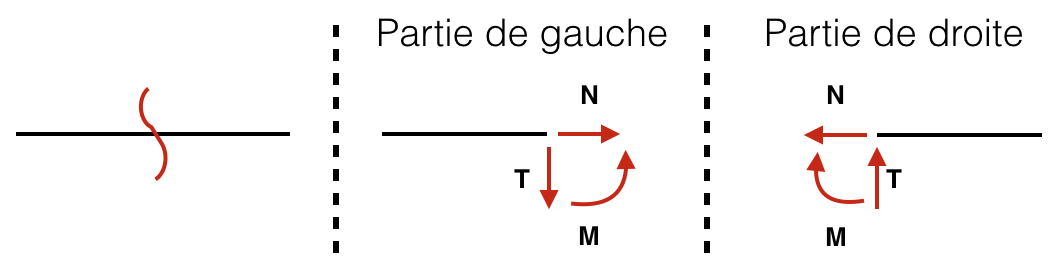
\includegraphics[scale=0.5]{Annexes/Rappels/1}
		\end{center}